\documentclass[letterpaper,11pt,leqno]{article}
\usepackage{paper}
\usepackage{listings}
\usepackage{xcolor}
\bibliographystyle{bibliography}

% Enter paper title to populate PDF metadata:
\hypersetup{pdftitle={Minimalist LaTeX Template for Academic Papers}}

% Enter path to BibTeX file with references:
\newcommand{\bib}{bibliography.bib}


\definecolor{codegreen}{rgb}{0,0.6,0}
\definecolor{codegray}{rgb}{0.5,0.5,0.5}
\definecolor{codepurple}{rgb}{0.58,0,0.82}
\definecolor{backcolour}{rgb}{0.95,0.95,0.92}

\lstdefinestyle{mystyle}{
    backgroundcolor=\color{backcolour},   
    commentstyle=\color{codegreen},
    keywordstyle=\color{magenta},
    numberstyle=\tiny\color{codegray},
    stringstyle=\color{codepurple},
    basicstyle=\ttfamily\footnotesize,
    breakatwhitespace=false,         
    breaklines=true,                 
    captionpos=b,                    
    keepspaces=true,                 
    numbers=left,                    
    numbersep=5pt,                  
    showspaces=false,                
    showstringspaces=false,
    showtabs=false,                  
    tabsize=2
}
\lstset{style=mystyle}


\newcommand{\pdf}{figures.pdf}

\begin{document}

% Enter title:
\title{Analiza podataka košarkaša Joel Embiid-a u R programskom jeziku}

% Enter authors:
\author{Adi Džombić}
%


% Enter date:
\date{\today}   

% Enter permanent URL (can be commented out):
\available{https://github.com/dzombicadi}

\begin{titlepage}
\maketitle

% Enter abstract:
Ovaj rad analizira perfomanse košarkaša Joel Embiid-a korištenjem stečenog znanja iz statistike i vjerovatnoće. Koristeći statističke alate i modele u R-u, istražujemo faktore koji utječu na ishode igre, kao što su učinkovitost igrača kao i ostale faktore koje utiču na njegovu igru. Putem metoda kao što su regresijska analiza i prediktivno modeliranje, cilj nam je otkriti obrasce koji mogu pružiti korisne uvide za poboljšanje izvedbe i optimizaciju strategija u košarci.

\end{titlepage}

% Enter main text:
\section{Uvod}\label{s:uvod}
 
\paragraph{Data Science} Integracija znanosti o podacima u sport revolucionirala je način na koji se igre analiziraju, razvijaju strategije i donose odluke. Košarka, sa svojom brzom akcijom i bogatim skupovima podataka, nudi savršenu arenu za primjenu tehnika znanosti o podacima. Ovo istraživanje usmjereno je na analizu podataka o košarci kako bi se otkrili obrasci i uvidi koji mogu poboljšati razumijevanje igre i informirati strateške odluke.

\paragraph{Cilj našeg istraživanja} Primarni cilj ovog rada je istraživanje različitih aspekata košarkašove igre kroz analizu podataka. Ključna područja fokusa uključuju procjenu učinka igrača, razumijevanje dinamike tima i identifikaciju faktora koji doprinose uspješnim ishodima igre. Koristeći statističke i računske tehnike, ova studija ima za cilj da izvuče značajne informacije iz neobrađenih skupova košarkaških podataka, pretvarajući ih u uvide koji se mogu primijeniti.

\section{Biblioteke i podaci koje koristimo}\label{s:section}

Podaci koje obrađujemo u ovom radu su prikupljeni od strane nekoliko košarkaških portala, te spakovani u jednostavnu R biblioteku pod nazivom "\textbf{nbastatR}" \footnote{https://www.rdocumentation.org/packages/nbastatR/}.
Biblioteka se sastoji od mnogobrojnih košarkaša, međutim zbog kratke dužine ovog kursa, obradit ćemo samo jednog igrača pod nazivom Joel Embiid \footnote{https://en.wikipedia.org/wiki/Embiid/}, usporediti njegovu igru sa par igrača njegovog nivoa i probat pronać razloge šta ga čini jednim od najboljih igrača u NBA današnjice.

Pored te biblioteke, iskoristit ću snagu "\textbf{Tidyverse}"\footnote{https://www.tidyverse.org/}
biblioteke. \textbf{Tidyverse je} kolekcija R biblioteka dizajniranih za obradu podataka, a razvili su je i održavali Hadley Wickham i RStudio tim. Izgrađen je oko strukture podataka nazvane "tibble", koja je slična podatkovnom okviru, ali s dodatnom funkcionalnošću. Tidyverse slijedi skup pravila nazvanih "tidy data" koji promoviraju strukturiran, lako razumljiv i učinkovit proces manipulacije podacima. Matematičari i analitičari podataka naširoko koriste ove principe i biblioteke u "tidyverse", čineći ga moćnim i praktičnim alatom za analizu podataka.

\newpage

\subsection{Pristup podacima o igraču}

Za početak instalirajmo prethodno navedene biblioteke za obradu podataka:

\begin{lstlisting}[language=R]
install.packages("nbastatR")
install.packages("tidyverse")
install.packages("tvthemes")

library(nbastatR)
library(tidyverse)
library(tvthemes)
\end{lstlisting}

Biblioteka "nbastatR" sadrži hiljade igrača... Potrebno je izdvojiti podatke našeg ciljanog igrača i njegove vrijednosti smjestiti u varijablu. To ćemo uraditi na sljedeći način:

\begin{lstlisting}[language=R]
Sys.setenv(VROOM_CONNECTION_SIZE=500072)

jojo_game_log <- suppressWarnings(
  game_logs( 
    seasons = c(2015:2023),
    league = "NBA", 
    result_types = "player",
    season_types = "Regular Season"))%>% 
filter(namePlayer == 'Joel Embiid')
\end{lstlisting}

Prva komanda proširuje default prostor varijable s obzirom da se radi o ogromnoj količini podataka. Veoma korisna stvar kod biblioteke "nbastatR" koju vrijedi napomenuti je da samo uz par linija koda, uspjeli smo "izvući" podatke iz njegovih 367 utakmica koje je odradio u periodu 2015-2023 godine.


\subsection{Prosjek poena po utakmici po sezoni} 

\begin{center}
    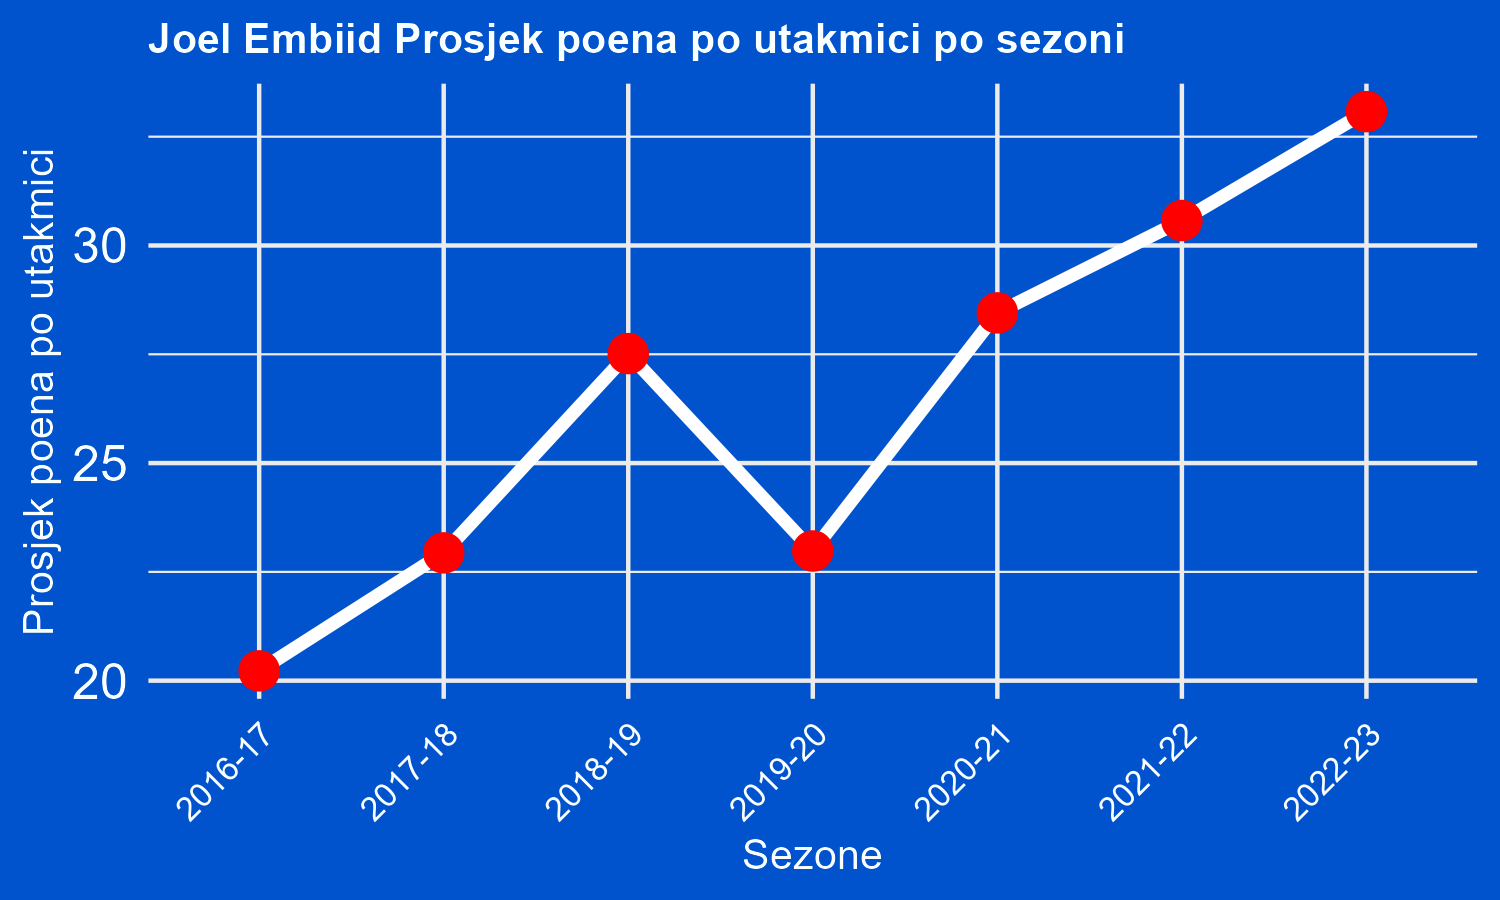
\includegraphics{AveragePoints.png}
\end{center}

Korištenjem sljedećeg koda dobili smo prethodni graf koji prikazuje prosjek poena po utakmici po sezoni našeg igrača. Ako pogledamo graf, možemo primijetiti da je prosjek poena drastično pao u sezoni 2019-2020. Nakon malo istraživanja, dolazimo do dva glavna razloga zbog ovakvog perfomansa u toj sezoni, a to su: ozljeda koljena i leđa, te pandemija COVID-19...

Ozljeda koljena je uzrokovala da propusti čak 22 utakmice\footnote{https://bit.ly/4iozfSp} tokom te sezone, ali sezone poslije te nastavlja da se konstantno poboljšava.

\begin{lstlisting}[language=R]
joel_points_per_season <- jojo_game_log %>%
  group_by(slugSeason) %>%
  summarise(avg_points = mean(as.numeric(pts), na.rm = TRUE)) %>%
  arrange(slugSeason)

ggplot(joel_points_per_season, aes(x = slugSeason, y = avg_points, group = 1)) +
  geom_line(color = "white", size = 1.5) +
  geom_point(color = "red", size = 4) +
  labs(
    title = "Joel Embiid Prosjek poena po utakmici po sezoni",
    x = "Sezone",
    y = "Prosjek poena po utakmici"
  ) +
  theme_brooklyn99() +
  theme(
    axis.text.x = element_text(angle = 45, hjust = 1, size = 8),
    plot.title = element_text(size = 10, face = "bold"),
    axis.title = element_text(size = 10)
  )

\end{lstlisting}

\subsection{Distribucija postotka šuteva}

Metrika koja nas takođe zanima je Joel Embiid-ov postotak šuta. Distribucije u nastavku pokazuju da on konstantno šutira preko 50\%. Kako mu je karijera napredovala, počeo je stalno pucati preko 60\%. Gledajući prosjek sezone, on je iznad 53,6\%, što je rekord karijere. Bez iznenađena, najmanji procenat šuteva je napravio u sezoni 2019-2020 zbog povrede.

\begin{lstlisting}[language=R]
jojo_game_log %>%
  ggplot(aes(x=slugSeason,y=round(pctFG*100,1))) +
  geom_jitter(color='#C4CED4')+
  geom_violin(alpha=.5,fill='#ED174C')+ 
  theme_brooklyn99()+
  theme(legend.position = 'none')+
  labs(x = "Sezone", y = "Postotak pogodaka na terenu") + 
  ggtitle('Distribucija procenta pogodaka')
\end{lstlisting}

\begin{center}
    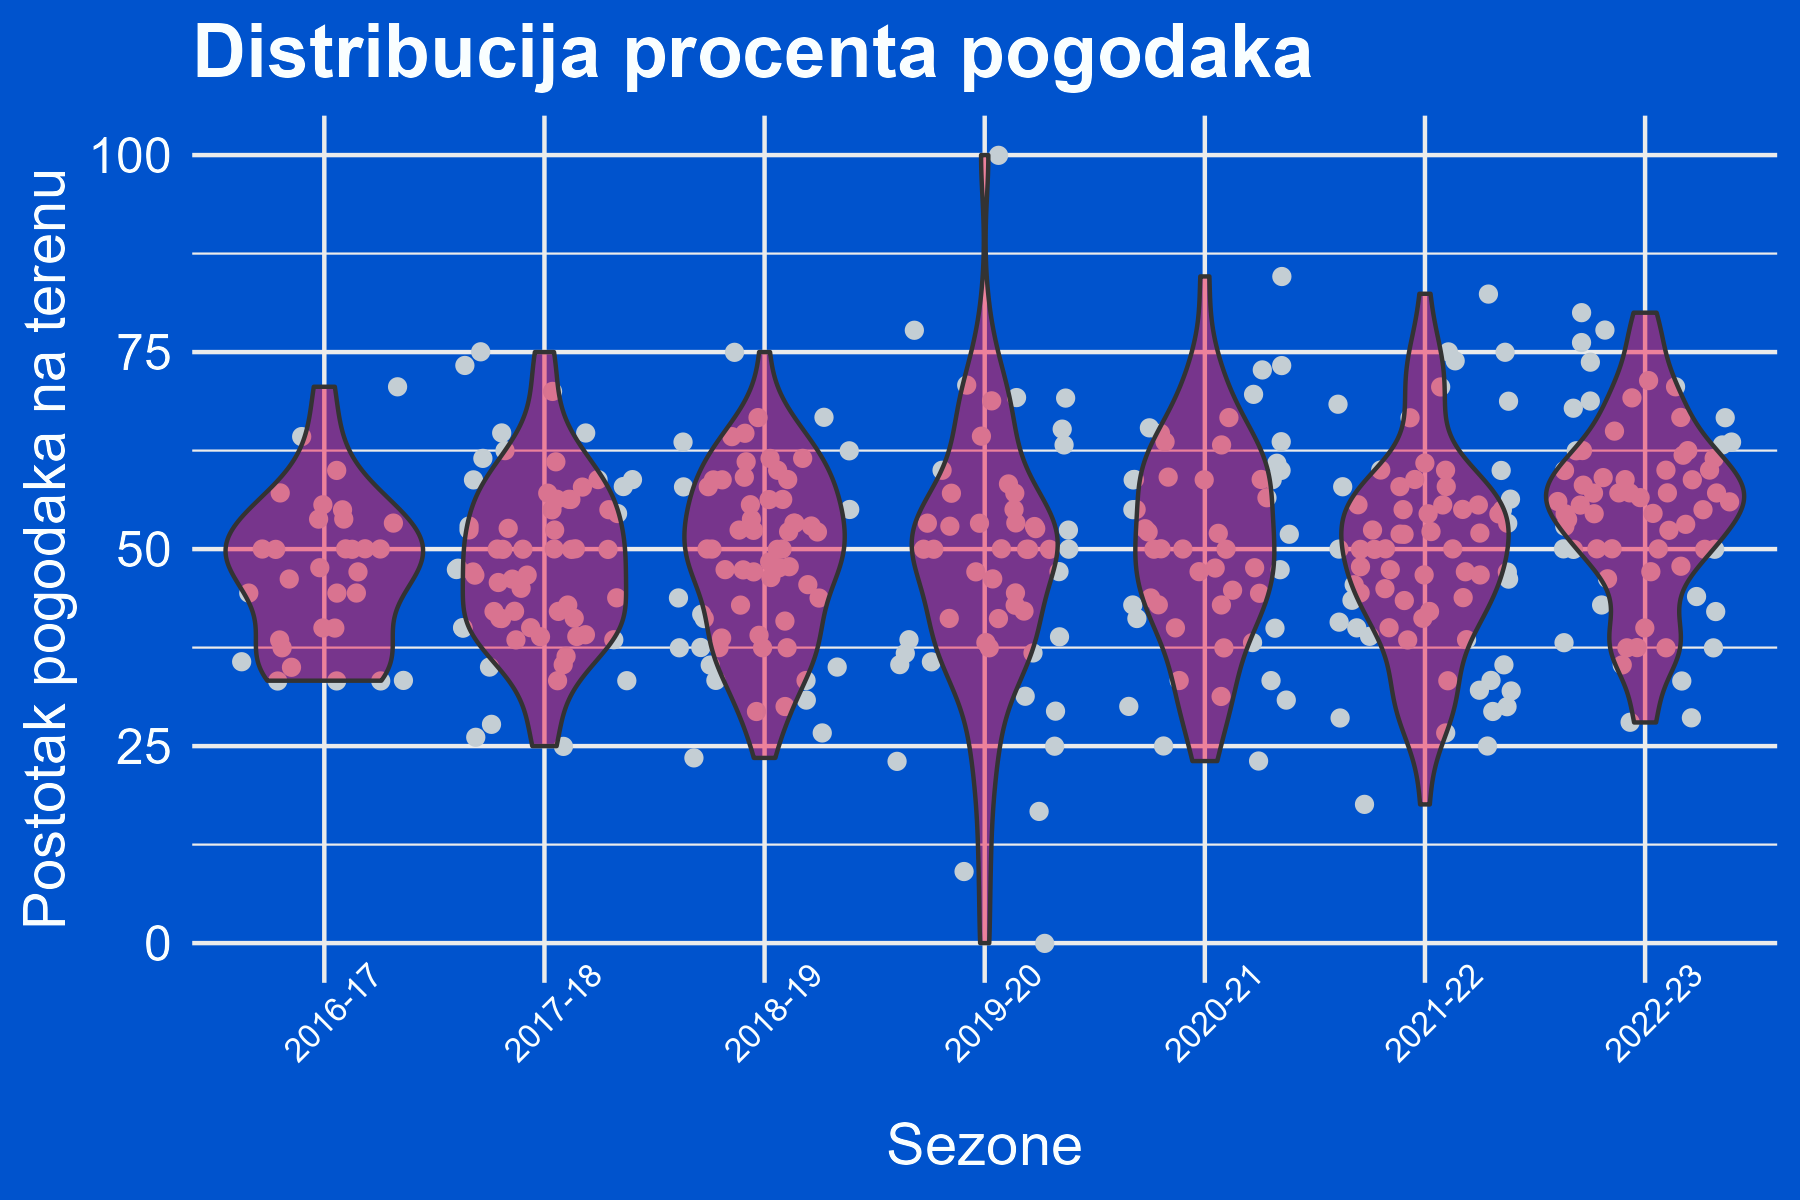
\includegraphics{DistribucijaPogodaka.png}
\end{center}


\subsection{Distribucija pogodaka za "tricu"}

Danas u košarci sve više igrača šutira trice. Visoki košarkaši nisu iznimka. Zapravo, ove sezone Joel Embiid je pokušao prosječno 3,25 šuteva za tricu po utakmici, malo niže nego u proteklih nekoliko sezona. Gledajući njegov postotak šuteva za tri poena, mnogo je manje konstantan.

\begin{lstlisting}[language=R]
jojo_game_log %>%
  ggplot(aes(x=slugSeason,y=round(pctFG3*100,1))) +
  geom_jitter(color = '#C4CED4')+
  geom_violin(alpha=.5,fill='#ED174C')+ 
  theme_brooklyn99()+
  theme(legend.position = 'none', axis.text.x = element_text(angle = 45))+
  labs(x = "Sezone", y = "Postotak pogodaka") + 
  ggtitle('Distribucija pogodaka za 3 poena')
\end{lstlisting}

\begin{center}
    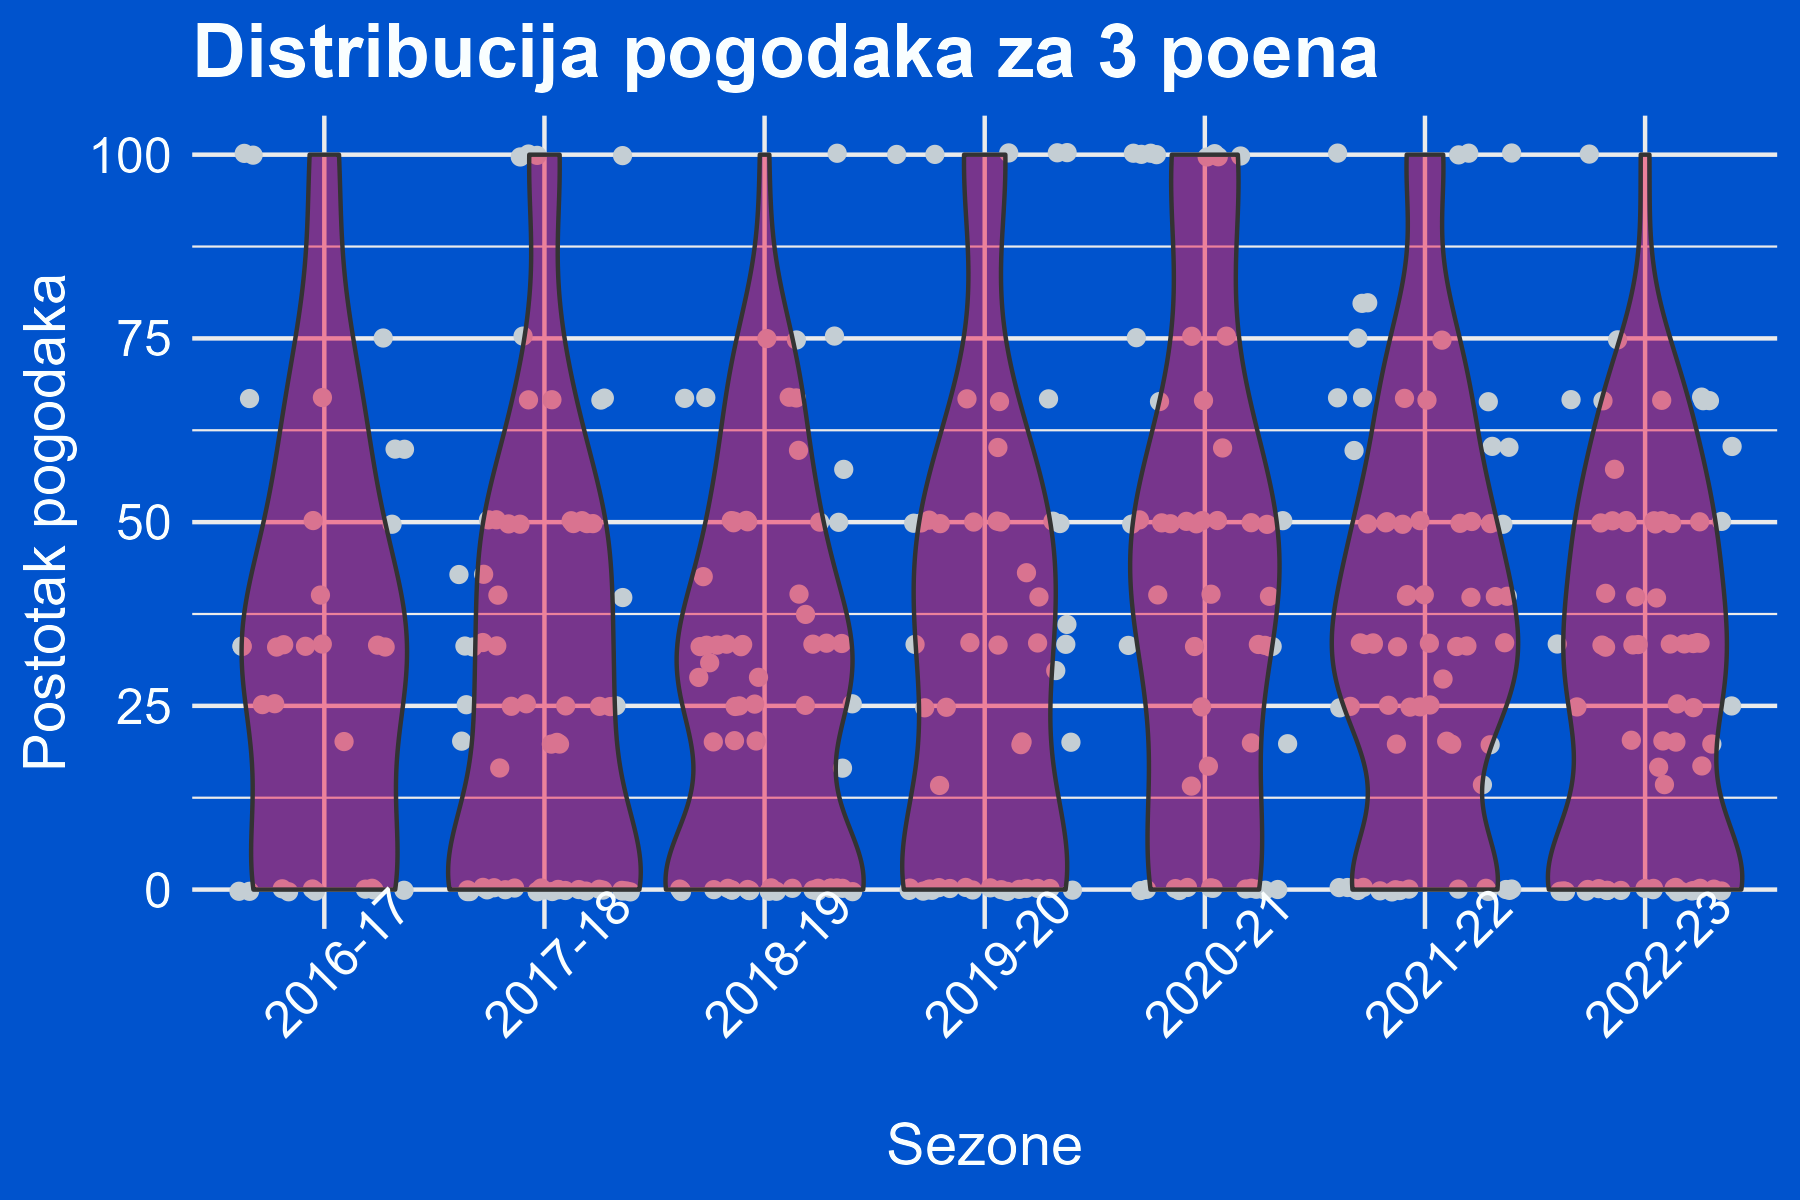
\includegraphics{DistribucijaTrica.png}
\end{center}

Iako iz utakmice u utakmicu prebacuje malo preko 3,25 šuteva za tricu, gledajući statistiku sezone, ostao je igrač koji pogađa 30\% šuteva za tri poena. Još jedan prikaz ovih rezultata možemo posmatrat sljedećim grafom:

\begin{lstlisting}[language=R]
jojo_game_log %>% 
  group_by(slugSeason) %>% 
  summarise(games_played = n(),
            avg_minutes_played = mean(minutes),
            fgm = sum(fg3m),
            fga = sum(fg3a)) %>% 
  mutate(fg_pct = fgm / fga) %>% 
  ggplot(aes(x = slugSeason, y = fg_pct)) + 
  geom_bar(stat = 'identity', fill = '#ED174C') + 
  theme_brooklyn99() + 
  theme(
    legend.position = 'none',
    axis.text.x = element_text(angle = 45, hjust = 1)
  ) + 
  labs(x = "Sezone", y = "Prosjek pogodaka") + 
  ggtitle("Distribucija pogodaka za 3 poena")
\end{lstlisting}

\begin{center}
    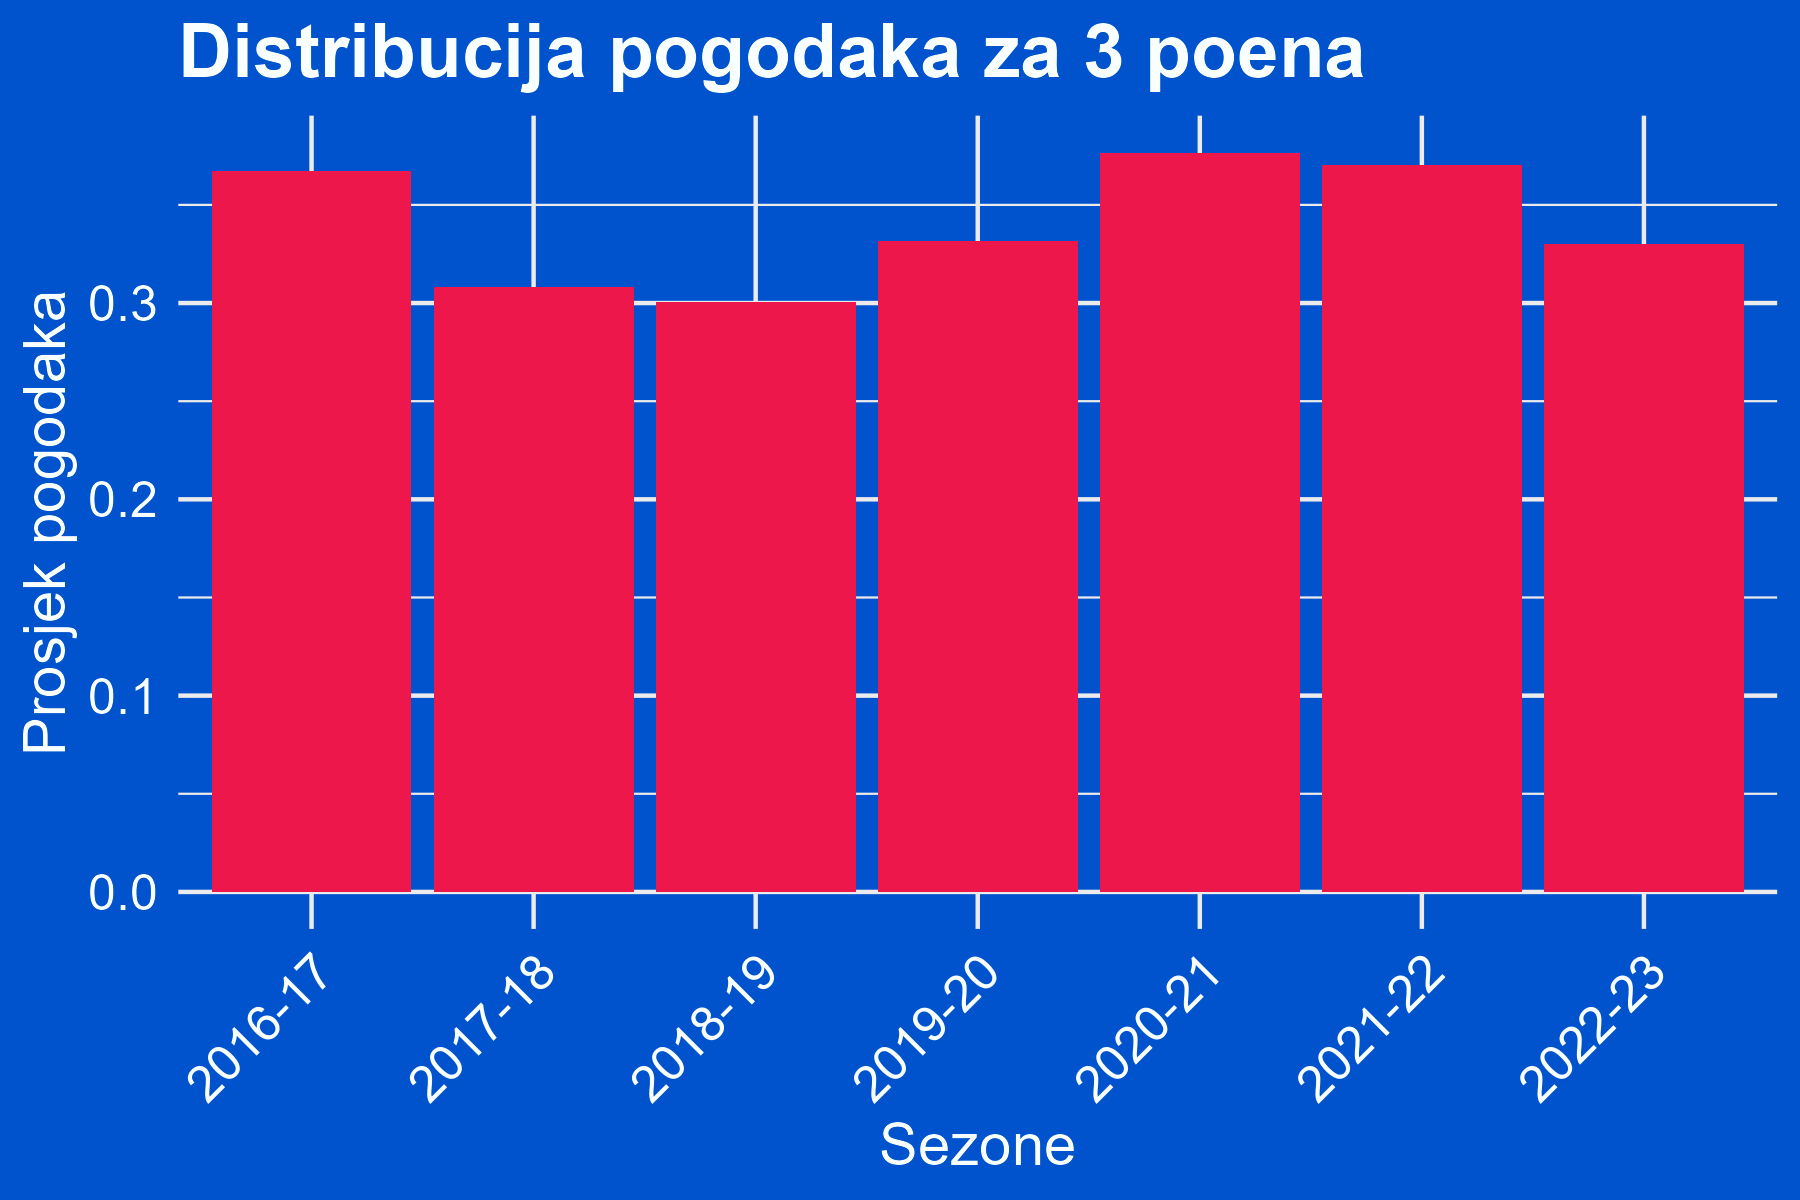
\includegraphics{DistribucijaTrica2.png}
\end{center}


\section{Usporedba Joel Embiid-a sa ostalim All-Star igračima}\label{s:math}

U ovom poglavlju poredit ćemo Joel Embiid-a sa ostalim All-Star igračima u 3 kategorije, a to su: prosjek pogodaka po utakmici u sezoni 2022-2023, prosjek bacanja na koš i prosjek pobjeda svakog igrača.

Prvo, moram izvući novi skup podataka pojedinih All-Stars igrača i Joel za sezonu 2022–2023. Srećom, biblioteka "nbastatsR" nam olakšava izvlačenje skupova podataka o igračima, timovima i sezonama.

\subsection{Izvlačenje podataka} 

Sa narednim kodom izvlačim statistiku 22–23 igrača i filtriram samo igrače iz All-Star tima i Joela Embiid-a:

\begin{lstlisting}[language=R]
all_stars = c('Giannis Antetokounmpo','Kevin Durant', 
            'Jayson Tatum' , 'Donovan Mitchell',
            'Kyrie Irving','LeBron James','Nikola Jokic',   
            'Zion Williamson' ,'Stephen Curry' , 
            'Luka Doncic','Joel Embiid')  

allStar_log <- suppressWarnings(
                game_logs(seasons = c(2023),
                          league = "NBA", 
                          result_types = "player", 
                          season_types = "Regular Season"))%>% 
              filter(namePlayer %in% all_stars)
\end{lstlisting}


\subsection{Prosjek pogodaka po utakmici u sezoni 2022-2023} 

Prva statistika koju sam pogledao bio je prosjek poena po utakmici. Joel zabija više poena po utakmici nego bilo koji od odabranih All Starsa. Naivno bi mogli zaključiti da je on jednostavno bolji od svih ostalih, međutim, može se desiti i da on "baca" na koš dosta više od svih ostalih košarkaša... Iz tog razloga je potrebno pogledati koji je njegov prosjek bacanja na koš u sljedećem poglavlju.

\begin{lstlisting}[language=R]
all_stars = c('Giannis Antetokounmpo','Kevin Durant', 
            'Jayson Tatum' , 'Donovan Mitchell',
            'Kyrie Irving','LeBron James','Nikola Jokic',   
            'Zion Williamson' ,'Stephen Curry' , 
            'Luka Doncic','Joel Embiid')  

allStar_log <- suppressWarnings(
                game_logs(seasons = c(2023),
                          league = "NBA", 
                          result_types = "player", 
                          season_types = "Regular Season"))%>% 
              filter(namePlayer %in% all_stars)
\end{lstlisting}

\begin{center}
    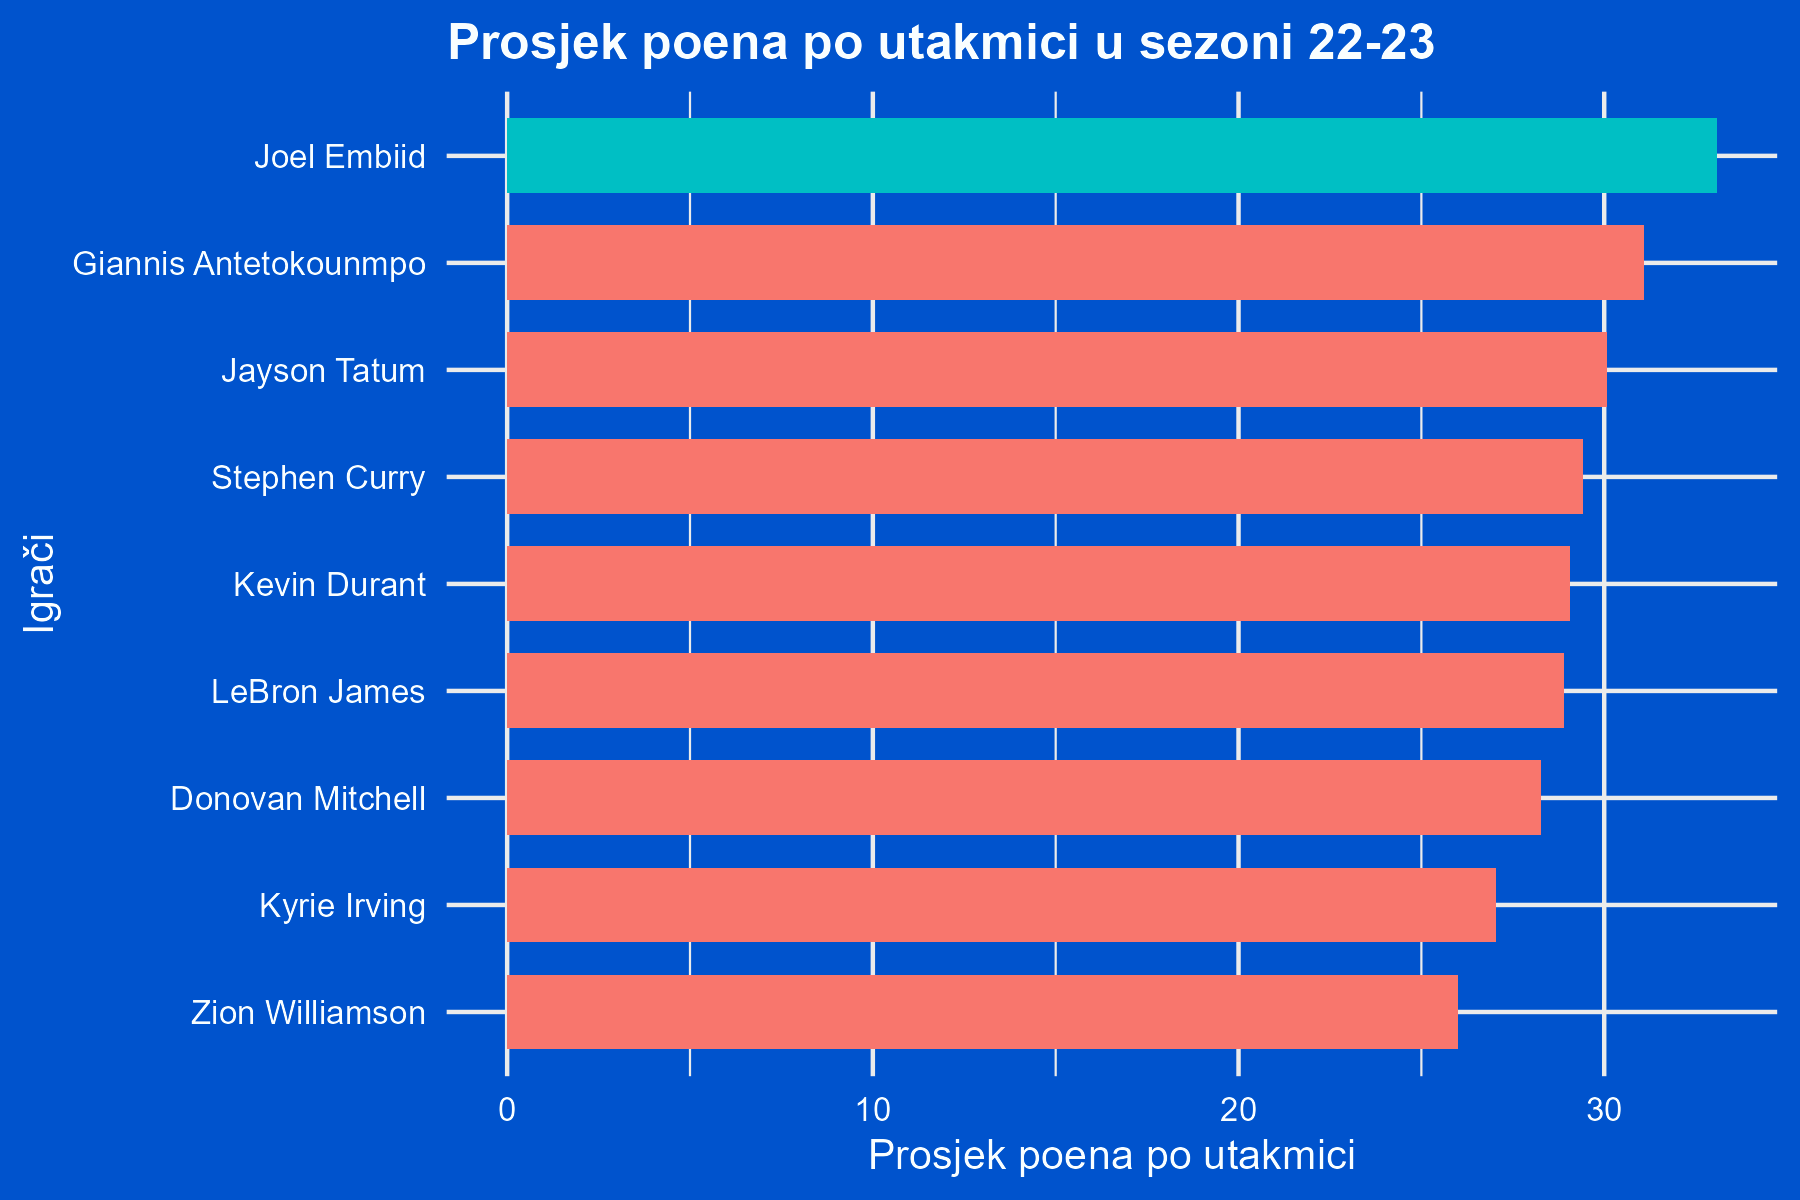
\includegraphics[scale=0.9]{ProsjekPoena22-23.png}
\end{center}

\subsection{Prosjek bacanja na koš}

Iako Joel nije na vrhu popisa, on ima bolji postotak od barem polovice All-Star igrača. Ipak, istok izgleda malo konkurentniji od zapada kada je riječ o ovoj statistici. Prosjek bacanja na koš dobijamo sljedećim kodom:

\begin{lstlisting}[language=R]
allStar_log %>% 
  group_by(namePlayer) %>% 
  summarise(games_played = n(),
            avg_minutes_played = mean(minutes),
            mean_points = mean(pts),
            fgm = sum(fgm),
            fga = sum(fga)) %>% 
  mutate(fg_pct = fgm / fga,
         all_star_starter = ifelse(namePlayer == 'Joel Embiid','Joel Embiid' , 'Starter')) %>% 
  ggplot(aes(x=reorder(namePlayer,fg_pct),y=fg_pct,fill=all_star_starter)) + 
  coord_flip()+
  geom_bar(stat='identity')+  
  theme_brooklyn99() + 
  labs(x = "Igraci", y = "Postotak bacanja") + 
  ggtitle('Prosjek bacanja na kos')
\end{lstlisting}

\begin{center}
    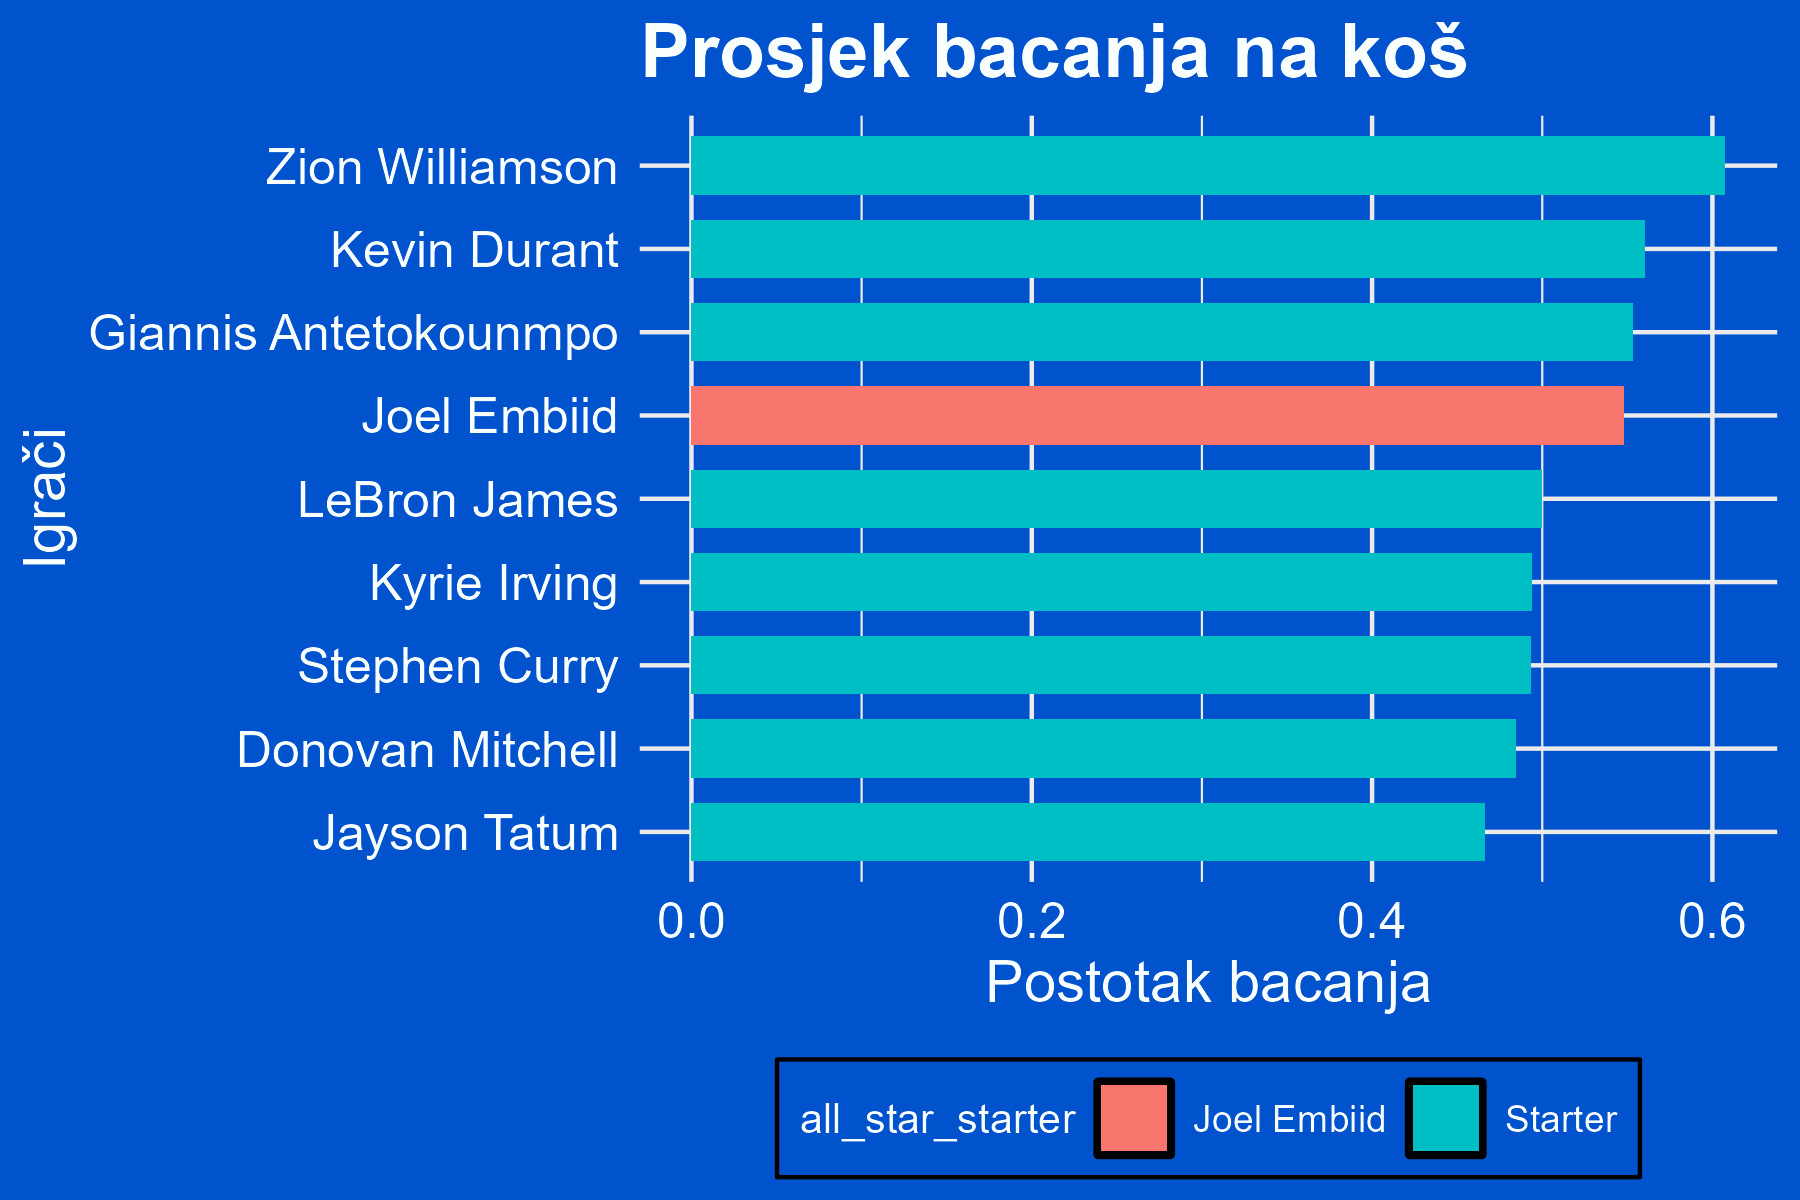
\includegraphics[scale=1]{ProsjekBacanja.png}
\end{center}

\subsection{Prosjek pobjeda u 2022-2023 sezoni} 

Konačno, koliki je postotak pobjeda ovih igrača. Ove sezone Sixersi su trenutno treći i prilično im dobro ide. Joel je bio ozlijeđen ranije tokom sezone, ali je ove sezone igrao onoliko minuta koliko je igrao u prethodnim sezonama. Njegov prosjek pobjeda je veći od 60\%, a samo nekoliko od svih All-Star igrača će vjerovatno imati veći prosjek od njega. Sljedećim kodom ćemo dobiti graf prosjeka pobjeda nekoliko igrača:

\begin{lstlisting}[language=R]
allStar_log %>% 
  group_by(namePlayer) %>% 
  summarise(games_played = n(),
            avg_minutes_played = mean(minutes),
            mean_points = mean(pts),
            fgm = sum(fgm),
            fga = sum(fga),
            win = sum(ifelse(isWin == TRUE , 1,0))) %>% 
  mutate(fg_pct = fgm / fga,
         win_pct = win / games_played,
         all_star_starter = ifelse(namePlayer == 'Joel Embiid','Not All Star' , 'Starter')) %>% 
  ggplot(aes(x=reorder(namePlayer,win_pct),
             y=win_pct, fill=all_star_starter)) + 
  coord_flip()+
  geom_bar(stat='identity', width = 0.7)+  
  theme_brooklyn99() + 
  labs(x = "Igraci", y = "Procenat pobjeda") + 
  ggtitle('Prosjek pobjeda')
\end{lstlisting}

\begin{center}
    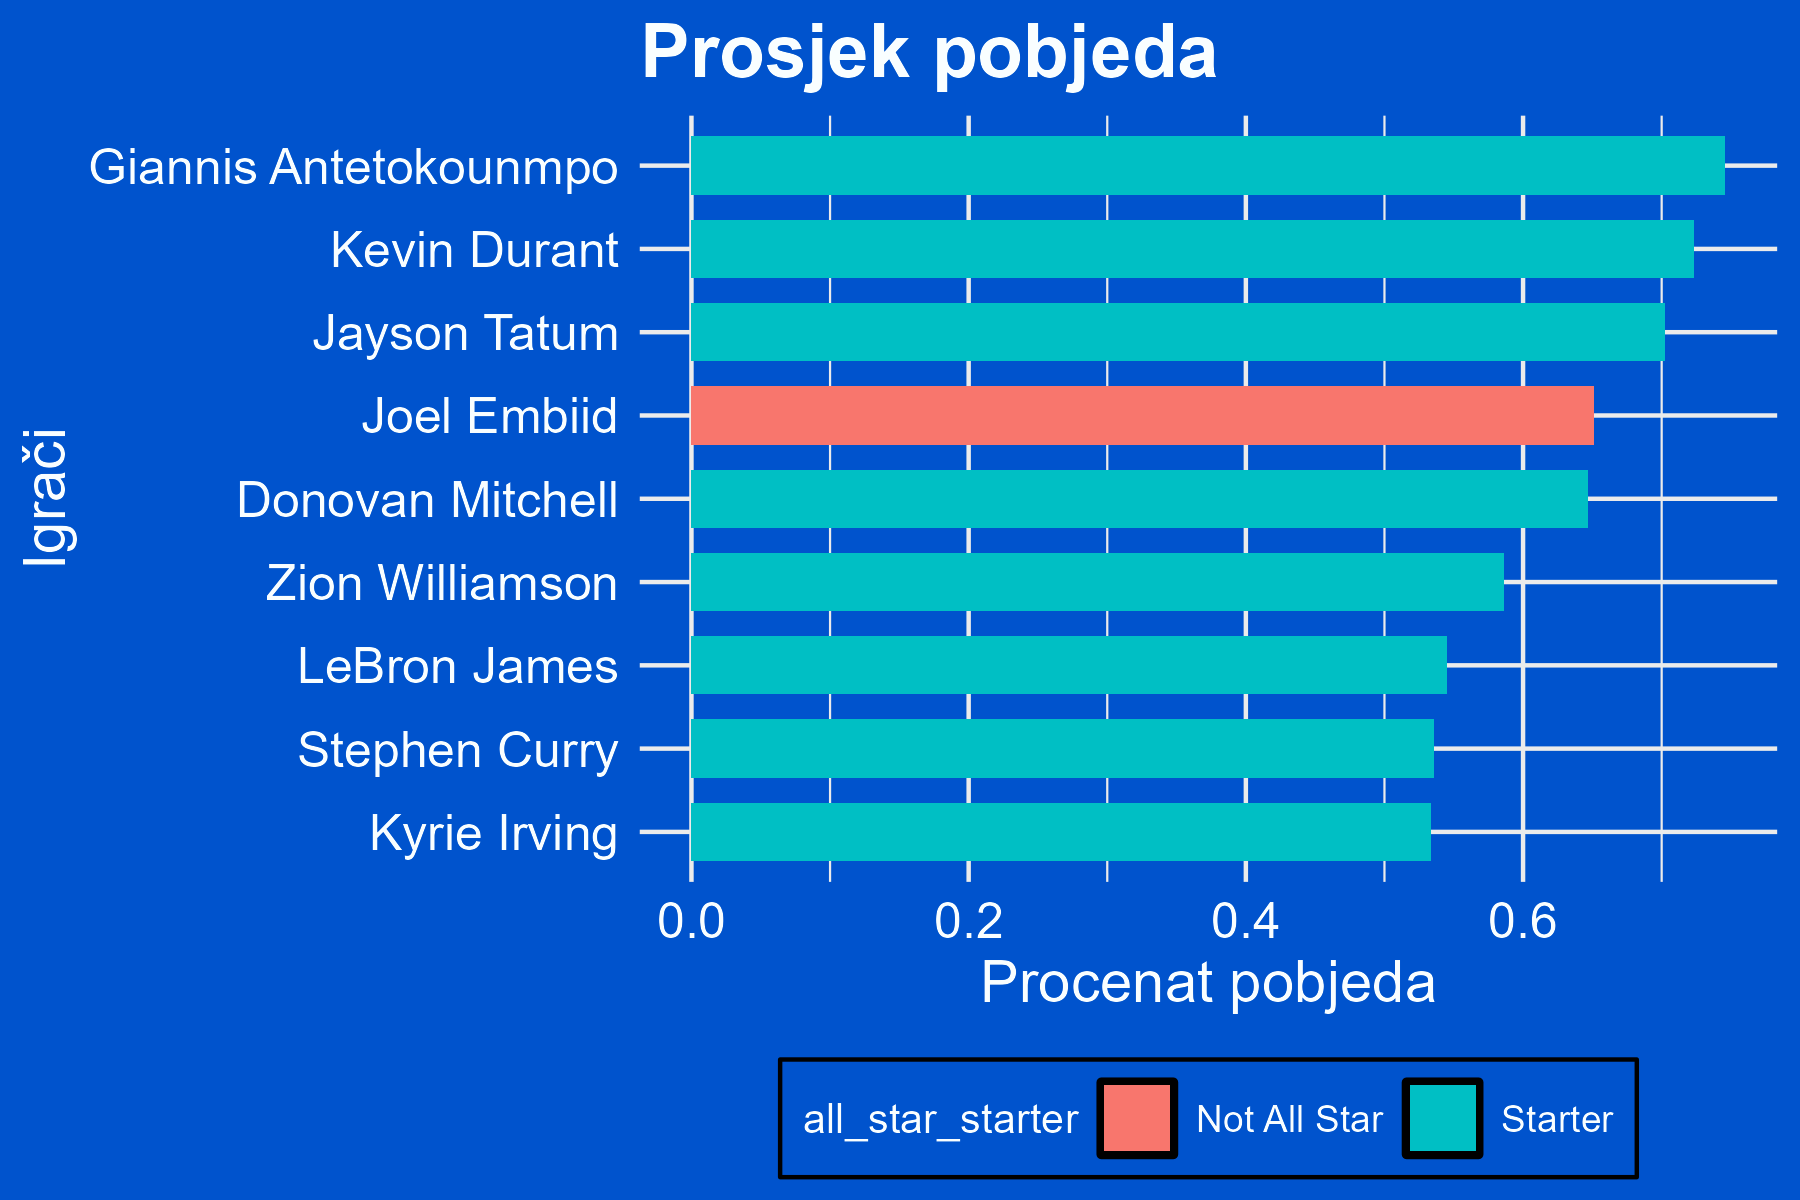
\includegraphics[scale=0.9]{ProcenatPobjeda.png}
\end{center}

\subsection{Nastavak...} 



\end{document}